\chapter{Beschreibung der verschiedenen Messungen und Ergbnisdarstellung}
% \section{ISDN-Dienste}%Fragen 3, 10
\section{Verbindungsauf- und abbau}%Namen �berdenken


%\clearpage
\begin{figure}[htbp] 
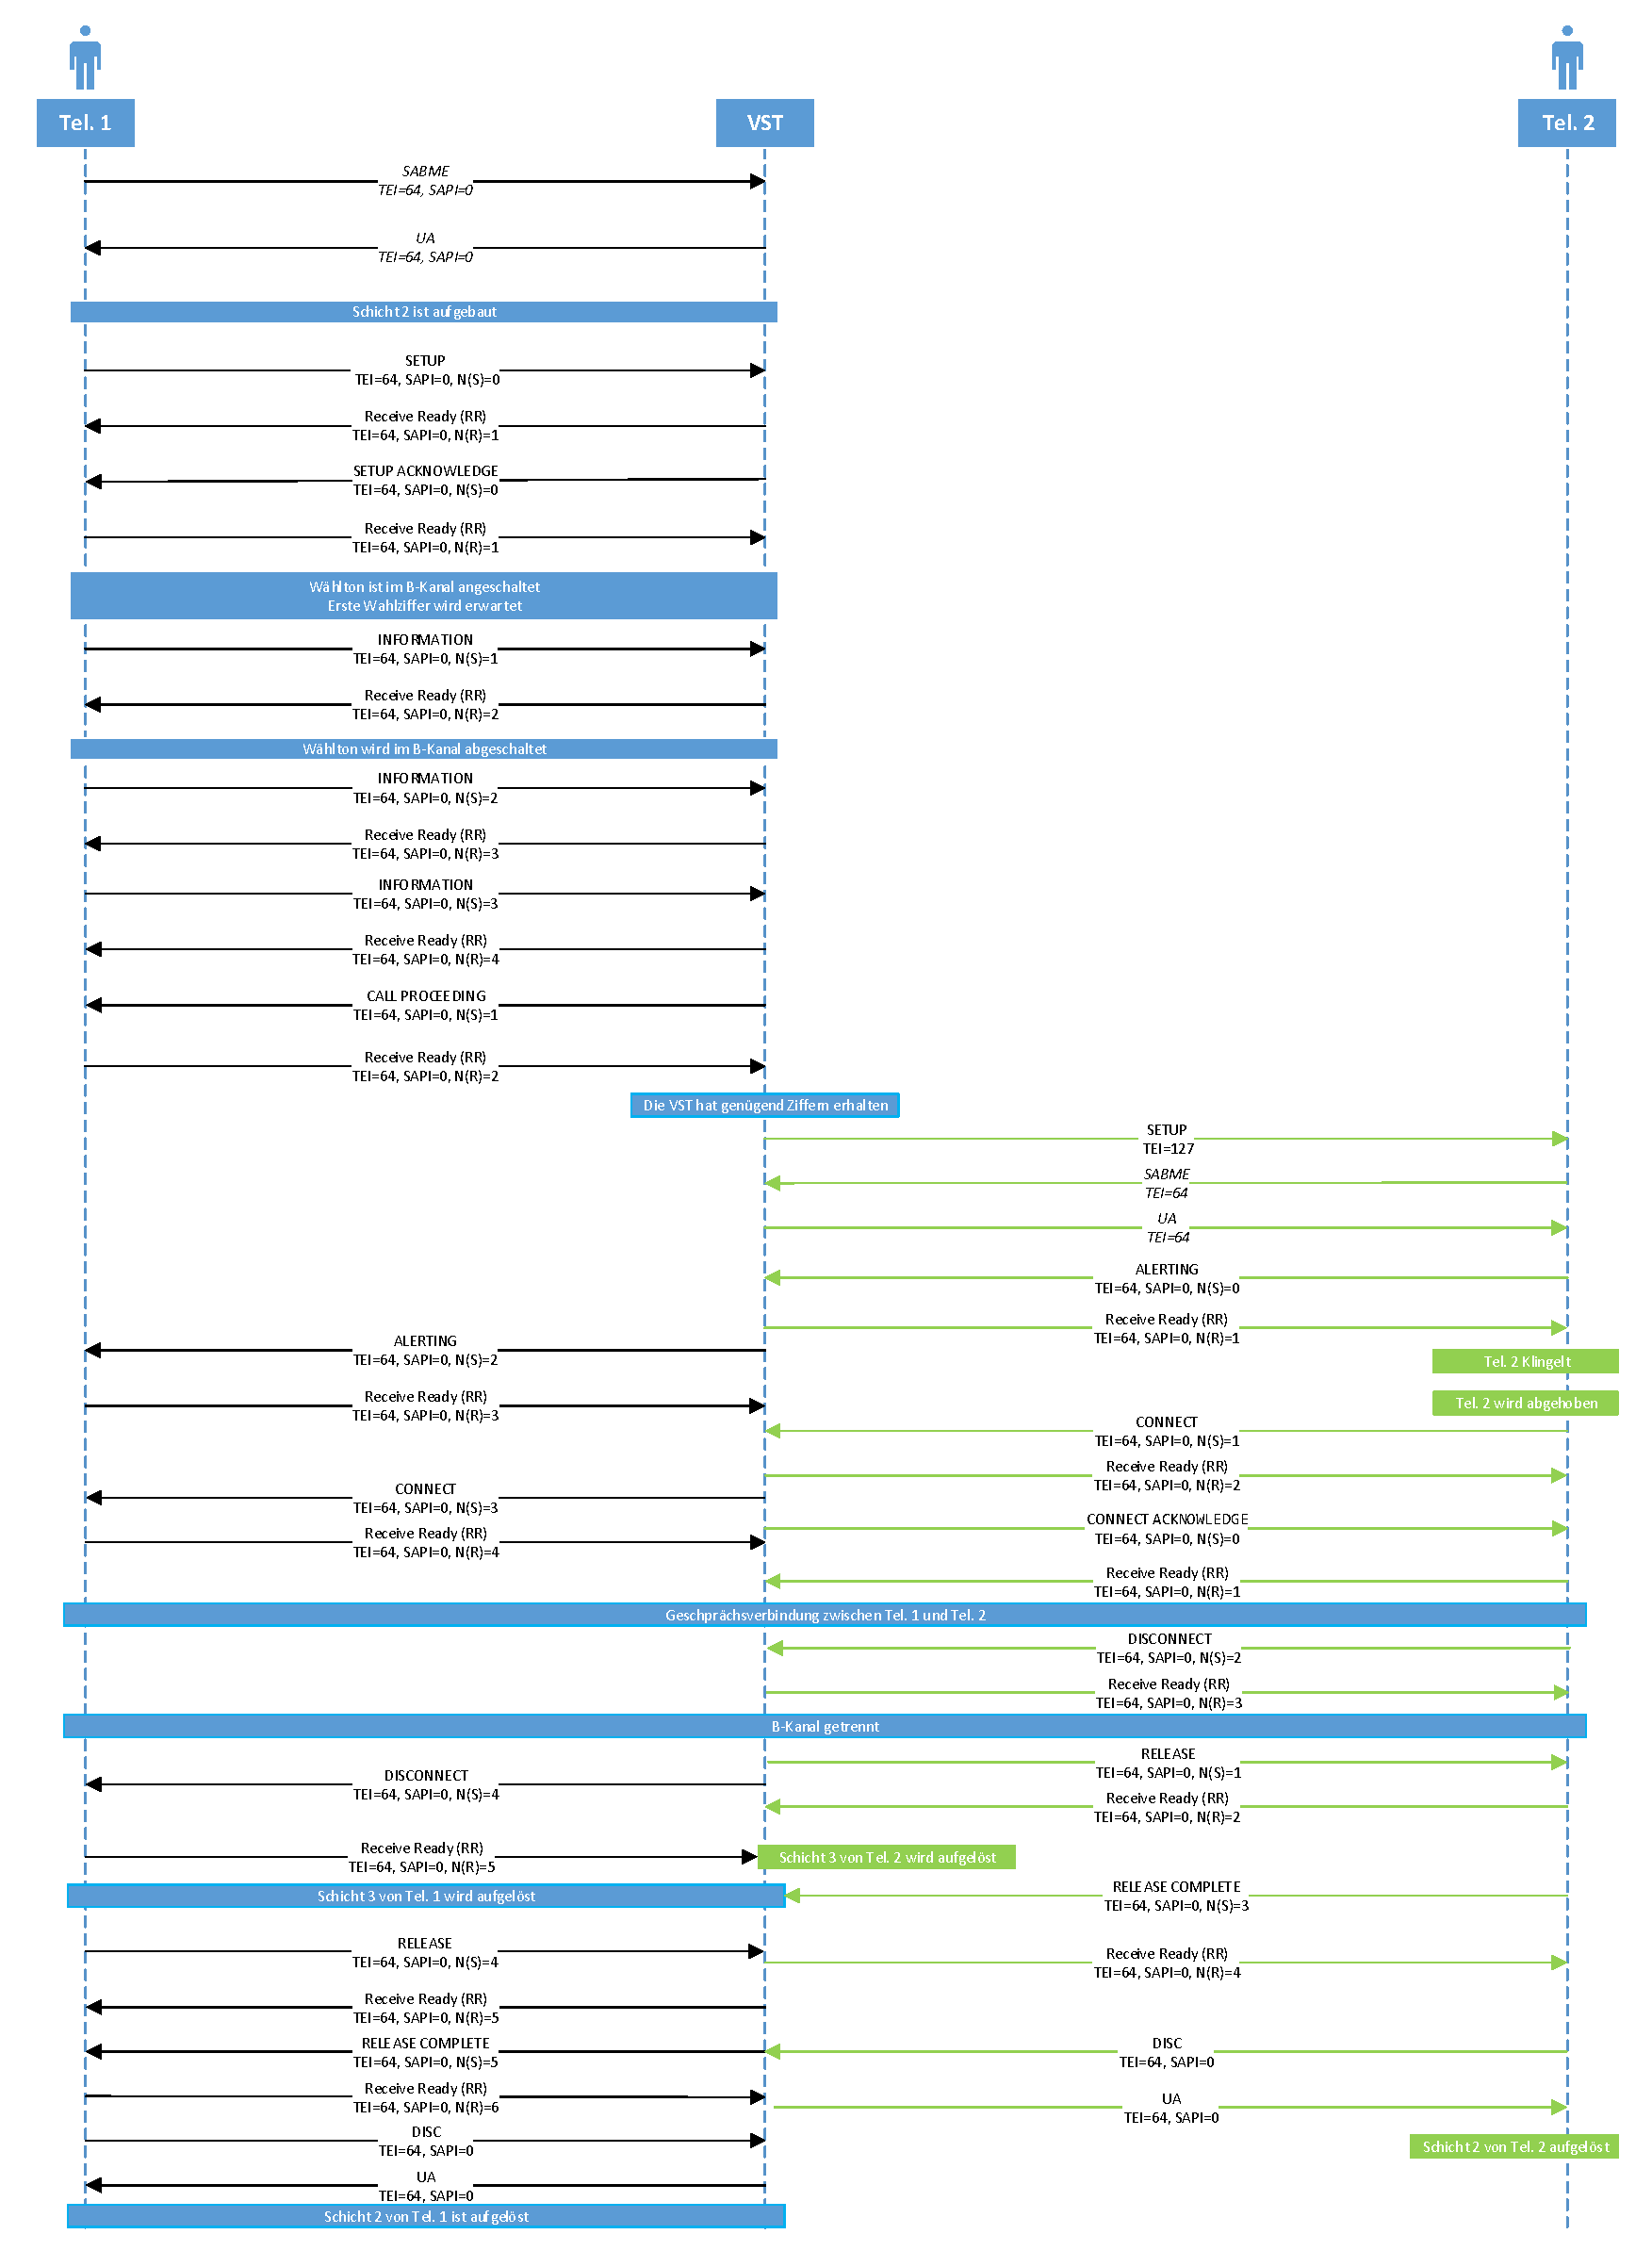
\includegraphics[width=\linewidth]{Graphics/KRAUS2}
\caption{Sequenzdiagramm zum Verbindungsauf- und abbau}
\label{fig:seq}
\end{figure}

Das Sequenzdiagramm zeigt den Ablauf des Verbindungsauf- und abbaus eines
Telefongespr�ches und wurde mit Hilfe des Wireshark-Protokllmitschnitts
erstellt. Aus dem Mitschnitt konnte der Nachrichtenverlauf zwischen Telefon 1
und der \ac{VSt} entnommen werden. Um die Kommunikation
zwischen Telefon 2 und der \acs{VSt} zu visualisieren wurde ``Die Technik der
Netze 1'' von Gerd Sigmund, als Quelle genutzt.\\%Quelle, S. 357-364
\newline
Im oberen Abschnitt wird die Schicht-2-Verbindung aufgebaut. Hierzu sendet das
Endger�t eine SABME-Nachricht, welche von der VSt mit einer UA-Nachricht
quittiert wird:
\begin{lstlisting}
No.     Time                       Source                Destination           Protocol Info
    338 2018-04-16 17:44:55.129216 User                  Network               LAPD     U P, func=SABME

Frame 338 (3 bytes on wire, 3 bytes captured)
    Arrival Time: Apr 16, 2018 17:44:55.129216000
    [Time delta from previous captured frame: 1561.020000000 seconds]
    [Time delta from previous displayed frame: 1561.020000000 seconds]
    [Time since reference or first frame: 24075.770216000 seconds]
    Frame Number: 338
    Frame Length: 3 bytes
    Capture Length: 3 bytes
    [Frame is marked: False]
    [Protocols in frame: isdn:lapd:data]
    Point-to-Point Direction: Sent (0)
ISDN
    Channel: D (0)
Link Access Procedure, Channel D (LAPD)
    [Direction: User->Network (0)]
    Address Field: 0x0081
        0000 00.. .... .... = SAPI: Q.931 Call control procedure (0)
        .... ..0. .... .... = C/R: 0
        .... ...0 .... .... = EA1: 0
        .... .... 1000 000. = TEI: 64
        .... .... .... ...1 = EA2: 1
    Control field: U P, func=SABME (0x7F)
        ...1 .... = Poll: Set
        011. 11.. = Command: Set Asynchronous Balanced Mode Extended (0x1b)
        .... ..11 = Frame type: Unnumbered frame (0x03)

No.     Time                       Source                Destination           Protocol Info
    339 2018-04-16 17:44:55.133216 Network               User                  LAPD     U F, func=UA

Frame 339 (3 bytes on wire, 3 bytes captured)
    Arrival Time: Apr 16, 2018 17:44:55.133216000
    [Time delta from previous captured frame: 0.004000000 seconds]
    [Time delta from previous displayed frame: 0.004000000 seconds]
    [Time since reference or first frame: 24075.774216000 seconds]
    Frame Number: 339
    Frame Length: 3 bytes
    Capture Length: 3 bytes
    [Frame is marked: False]
    [Protocols in frame: isdn:lapd:data]
    Point-to-Point Direction: Received (1)
ISDN
    Channel: D (0)
Link Access Procedure, Channel D (LAPD)
    [Direction: Network->User (1)]
    Address Field: 0x0081
        0000 00.. .... .... = SAPI: Q.931 Call control procedure (0)
        .... ..0. .... .... = C/R: 0
        .... ...0 .... .... = EA1: 0
        .... .... 1000 000. = TEI: 64
        .... .... .... ...1 = EA2: 1
    Control field: U F, func=UA (0x73)
        ...1 .... = Final: Set
        011. 00.. = Response: Unnumbered Acknowledge (0x18)
        .... ..11 = Frame type: Unnumbered frame (0x03)
\end{lstlisting}

Der Austausch dieser Nachrichten ist zeit�berwacht. Sende- und
Empfangsz�hler werden an dieser Stelle zur�ckgesetzt. Nach dem erfolgreichen
Aufbau der Schicht 2 k�nnen nummerierte I-Bl�cke ausgetauscht werden. Diese sind
mit Z�hlernummern versehen: N(S), die gesendeten Bl�cke, und N(R), die
empfangenen Bl�cke.\\
\newline
Der Aufbau der Schicht 3 beginnt mit der SETUP-Nachricht und findet im
Anschluss, bei bestehender Schicht-2-Verbindung, statt. Mit Senden der
CONNECT ACKNOWLEDGE ist der Aufbau dre Schicht 3
abgeschlossen. Diese Nachricht dient zur Best�tigung, dass der angerufene
Teilnehmer die Verbindung angenommen hat (H�rer abgenommen). Danach wird der
B-Kanal im Netz durchgeschaltet, welcher zuvor mit der CONN ACK zugewiesen
wurde.\\
In diesem Versuch wurde der B-Kanal 1 zugewiesen. Dies ist der letzten Zeile des
folgenden Frames zu entnehmen:
\begin{lstlisting}
No.     Time                       Source                Destination           Protocol Info
    342 2018-04-16 17:44:55.177168 Network               User                  Q.931    SETUP ACKNOWLEDGE

Frame 342 (11 bytes on wire, 11 bytes captured)
    Arrival Time: Apr 16, 2018 17:44:55.177168000
    [Time delta from previous captured frame: 0.007984000 seconds]
    [Time delta from previous displayed frame: 0.007984000 seconds]
    [Time since reference or first frame: 24075.818168000 seconds]
    Frame Number: 342
    Frame Length: 11 bytes
    Capture Length: 11 bytes
    [Frame is marked: False]
    [Protocols in frame: isdn:lapd:q931]
    Point-to-Point Direction: Received (1)
ISDN
    Channel: D (0)
Link Access Procedure, Channel D (LAPD)
    [Direction: Network->User (1)]
    Address Field: 0x0281
        0000 00.. .... .... = SAPI: Q.931 Call control procedure (0)
        .... ..1. .... .... = C/R: 1
        .... ...0 .... .... = EA1: 0
        .... .... 1000 000. = TEI: 64
        .... .... .... ...1 = EA2: 1
    Control field: I, N(R)=1, N(S)=0 (0x0200)
        0000 001. .... .... = N(R): 1
        .... .... 0000 000. = N(S): 0
        .... .... .... ...0 = Frame type: Information frame (0x0000)
Q.931
    Protocol discriminator: Q.931
    Call reference value length: 1
    Call reference flag: Message sent to originating side
    Call reference value: 01
    Message type: SETUP ACKNOWLEDGE (0x0d)
    Channel identification
        Information element: Channel identification
        Length: 1
        1... .... = Extension indicator: last octet
        .0.. .... = Interface identifier present: False
        ..0. .... = Interface type: Basic rate interface
        .... 1... = Indicated channel is exclusive: Exclusive; only the indicated channel is acceptable
        .... .0.. = D-channel indicator: False
        .... ..01 = Information channel selection: B1 channel (0x01)
\end{lstlisting}

Im Mitschnitt dieses Versuchs wird die oben genannte CONNECT ACKNOWLEDGE nicht
aufgef�hrt, da wir aufgrund des Versuchsaufbaus nur die Nachrichten der
anrufenden Seite aufzeichnen konnten. Es w�re auch m�glich, dass
die CONNECTION ACKNOWLEDGE vom Telefon 1 zur \acs{VSt} gesendet wird. Da die
Nachricht aber in diesem Fall keine Beduetung hat, kann diese, wie im
Protokollmitschnitt, entfallen.\\%S.311 
\newline
Nachdem der H�rer von Telefon 2 aufgelegt wurde, wird eine DISCONNECT-Nachricht
gesendet, welche den Abbau der Schicht-3-Verbindung einleitet. Durch die
im Anschluss folgende RELEASE COMPLETE Nachricht ist die Schicht-3-Verbindung
abgebaut.\\Danach wird die Schicht 2 abgebaut, dies geschieht durch eine
DISC-Nachricht, welche mit einer UA quittiert wird.
%TODO Quelle

\section{Adressierung der Endger�te}\label{tei}
Im Adressfeld des HDLC-Protokolls befindet sich der \ac{TEI}. Jedem Endger�t ist
ein solcher Identifier zugeordnet um eine logische Verbindung zwischen
Vermittlungsstelle und Endger�t sicherzustellen. Der TEI kennzeichnet die
Schicht-2-Adresse f�r das ISDN-Ger�t.\\%TODO Quelle: Net_IT, s.325
Der TEI-Wert kann entweder durch manuelle Einstellung am Ger�t hinterlegt werden
oder von der Vermittlungsstelle zugeteilt werden (TEI-Vergabe). In diesem
Versuch stellt das Endger�t zuerst eine Identity Request, worauf die
Vermittlungsstelle bei Erfolg mit Identity Assigned antwortet. Die Vergabe
erfolgt mittels U-Frame.%TODO: mehr
Dem Ger�t wird der TEI 64 zugeteilt. Dies ist der erste von der
Vermittlungsstelle zu vergebende Wert. Die Adressen 1-63 k�nnen eingestellt
werden, 64-126 werden von der Vermittlungsstelle verteilt. TEI 127 stellt die
Broadcast-Adresse dar.
\newline
\ac{SAPI} bezeichnet ein weiteres Element des HDLC-Adressfeldes und kennzeichnet
den momentan verwendeten ISDN-Schicht-2-Dienst.%TODO Quelle: siehe oben,s.326
Bei der TEI-Vergabe ist der Wert des SAPI 63. Dem Protokoll zufolge bedeutet
dies ``Layer 2 management procedures''. Es handelt sich hier um die �bertragung
von paketvermittelten Daten.%TODO Qzelle identisch

%TODO Zeilennummerierung

\begin{lstlisting}

No.     Time                       Source                Destination           Protocol Info
     56 2018-04-16 16:30:58.999168 User                  Network               TEI      Identity Request

Frame 56 (8 bytes on wire, 8 bytes captured)
    Arrival Time: Apr 16, 2018 16:30:58.999168000
    [Time delta from previous captured frame: 2.003968000 seconds]
    [Time delta from previous displayed frame: 2.003968000 seconds]
    [Time since reference or first frame: 19639.640168000 seconds]
    Frame Number: 56
    Frame Length: 8 bytes
    Capture Length: 8 bytes
    [Frame is marked: False]
    [Protocols in frame: isdn:lapd:tei_management]
    Point-to-Point Direction: Sent (0)
ISDN
    Channel: D (0)
Link Access Procedure, Channel D (LAPD)
    [Direction: User->Network (0)]
    Address Field: 0xfcff
        1111 11.. .... .... = SAPI: Layer 2 management procedures (63)
        .... ..0. .... .... = C/R: 0
        .... ...0 .... .... = EA1: 0
        .... .... 1111 111. = TEI: 127
        .... .... .... ...1 = EA2: 1
    Control field: U, func=UI (0x03)
        000. 00.. = Command: Unnumbered Information (0x00)
        .... ..11 = Frame type: Unnumbered frame (0x03)
TEI Management Procedure, Channel D (LAPD)

No.     Time                       Source                Destination           Protocol Info
     57 2018-04-16 16:30:59.005200 Network               User                  TEI      Identity Assigned

Frame 57 (8 bytes on wire, 8 bytes captured)
    Arrival Time: Apr 16, 2018 16:30:59.005200000
    [Time delta from previous captured frame: 0.006032000 seconds]
    [Time delta from previous displayed frame: 0.006032000 seconds]
    [Time since reference or first frame: 19639.646200000 seconds]
    Frame Number: 57
    Frame Length: 8 bytes
    Capture Length: 8 bytes
    [Frame is marked: False]
    [Protocols in frame: isdn:lapd:tei_management]
    Point-to-Point Direction: Received (1)
ISDN
    Channel: D (0)
Link Access Procedure, Channel D (LAPD)
    [Direction: Network->User (1)]
    Address Field: 0xfeff
        1111 11.. .... .... = SAPI: Layer 2 management procedures (63)
        .... ..1. .... .... = C/R: 1
        .... ...0 .... .... = EA1: 0
        .... .... 1111 111. = TEI: 127
        .... .... .... ...1 = EA2: 1
    Control field: U, func=UI (0x03)
        000. 00.. = Command: Unnumbered Information (0x00)
        .... ..11 = Frame type: Unnumbered frame (0x03)
TEI Management Procedure, Channel D (LAPD)
\end{lstlisting}

 %ITU T I.241.1

\section{W�hlvorgang und Rufnummer�bertragung}%Frage 5, 8, 9, 12
Es gibt zwei M�glichkeiten beim Anruf die Rufnummer (\ac{MSN}) einzugeben.
Beim Versuch, der im Diagramm \label{seq} dargestellt ist, wurde zun�chst der H�rer
abgenommen und dann die Zielrufnummer eingegeben.\\Bei der zweiten Variante wird
zuerst die Rufnummer vollst�ndig eingegeben bevor der H�rer abgenommen wird.
Dieser W�hlvorgang wird Blockwahl genannt.\\
\newline
Bei der normalen Wahl werden die Ziffern der Rufnummer in einzelnen
Info-Nachrichten �bertragen:
%TODO Ausschnitt
Bei der Blockwahl hingegeben ist die \acs{MSN} des Ziels direkt bekannt und wird
in der SETUP-Nachricht �bertragen:
\begin{lstlisting}
No.     Time                       Source                Destination           Protocol Info
    366 2018-04-16 17:56:17.227216 User                  Network               Q.931    SETUP

Frame 366 (30 bytes on wire, 30 bytes captured)
    Arrival Time: Apr 16, 2018 17:56:17.227216000
    [Time delta from previous captured frame: 0.034000000 seconds]
    [Time delta from previous displayed frame: 0.034000000 seconds]
    [Time since reference or first frame: 24757.868216000 seconds]
    Frame Number: 366
    Frame Length: 30 bytes
    Capture Length: 30 bytes
    [Frame is marked: False]
    [Protocols in frame: isdn:lapd:q931]
    Point-to-Point Direction: Sent (0)
ISDN
    Channel: D (0)
Link Access Procedure, Channel D (LAPD)
    [Direction: User->Network (0)]
    Address Field: 0x0081
        0000 00.. .... .... = SAPI: Q.931 Call control procedure (0)
        .... ..0. .... .... = C/R: 0
        .... ...0 .... .... = EA1: 0
        .... .... 1000 000. = TEI: 64
        .... .... .... ...1 = EA2: 1
    Control field: I, N(R)=0, N(S)=0 (0x0000)
        0000 000. .... .... = N(R): 0
        .... .... 0000 000. = N(S): 0
        .... .... .... ...0 = Frame type: Information frame (0x0000)
Q.931
    Protocol discriminator: Q.931
    Call reference value length: 1
    Call reference flag: Message sent from originating side
    Call reference value: 01
    Message type: SETUP (0x05)
    Bearer capability
        Information element: Bearer capability
        Length: 3
        1... .... = Extension indicator: last octet
        .00. .... = Coding standard: ITU-T standardized coding (0x00)
        ...0 0000 = Information transfer capability: Speech (0x00)
        1... .... = Extension indicator: last octet
        .00. .... = Transfer mode: Circuit mode (0x00)
        ...1 0000 = Information transfer rate: 64 kbit/s (0x10)
        1... .... = Extension indicator: last octet
        .01. .... = Layer identification: Layer 1 identifier (0x01)
        ...0 0011 = User information layer 1 protocol: Recommendation G.711 A-law (0x03)
    Calling party number: '100'
        Information element: Calling party number
        Length: 5
        .... 0000 = Numbering plan: Unknown (0x00)
        .000 .... = Number type: Unknown (0x00)
        0... .... = Extension indicator: information continues through the next octet
        .... ..00 = Screening indicator: User-provided, not screened (0x00)
        .00. .... = Presentation indicator: Presentation allowed (0x00)
        1... .... = Extension indicator: last octet
        Calling party number digits: 100
    Called party number: '200'
        Information element: Called party number
        Length: 4
        .... 0001 = Numbering plan: E.164 ISDN/telephony numbering (0x01)
        .000 .... = Number type: Unknown (0x00)
        1... .... = Extension indicator: last octet
        Called party number digits: 200
        E.164 Called party number digits: 200
    High-layer compatibility
        Information element: High-layer compatibility
        Length: 2
        .00. .... = Coding standard: ITU-T standardized coding (0x00)
        High layer characteristics identification: Telephony
\end{lstlisting}

Diesbez�glich unterscheidet sich die SETUP-Nachricht bei den unterschiedlich
W�hlvorg�ngen. Beim normal W�hlverfahren ist die ``Called Party Number'' kein
Element der Nachricht, da die Nummer zu diesem Zeitpunkt nur bei der Blockwahl
bekannt ist.

\section{Nachrichtenelemente}

\begin{figure}[htbp] 
  \centering
     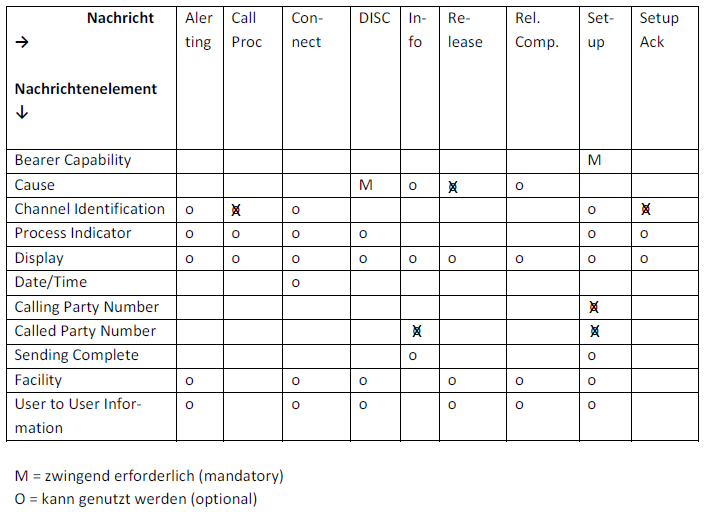
\includegraphics[width=\linewidth]{Graphics/Capture.PNG}
  \caption{Nachrichtenelemente}
  \label{fig:elemente}
\end{figure}
